
\chapter{MODELING AND DESIGN}
\section{\normalsize{\textbf{UML diagrams and DFDs}}}
\subsection{\normalsize{\textbf{Data Flow Diagrams}}}
\begin{itemize}
\item \textbf {DFD Level 0}
\end{itemize}
\begin{figure}[ht!]
	\centering
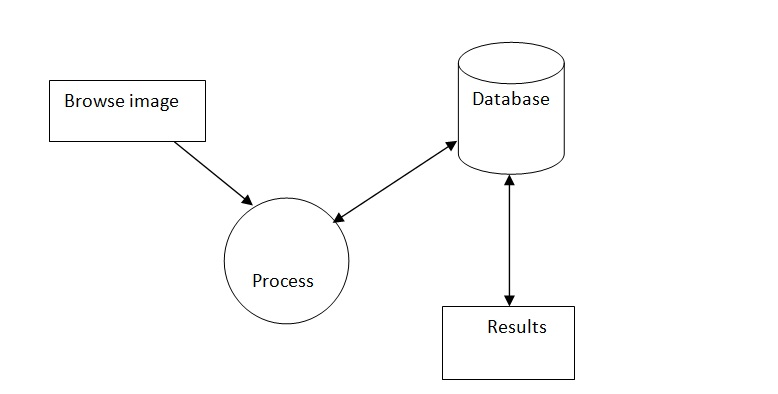
\includegraphics[height=250pt,width=435pt]{dfd0.jpg}\\
\caption{DFD Level-0}
\end{figure}
\newpage
\begin{itemize}
\item \textbf {DFD Level 1}
\end{itemize}
\begin{figure}[ht!]
	\centering
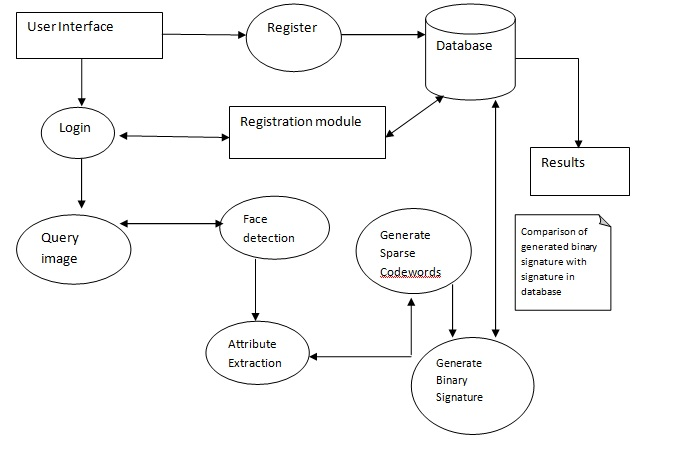
\includegraphics[height=250pt,width=435pt]{dfd1.jpg}\\
\caption{DFD Level-1}
\end{figure}
\subsection{UML Diagrams}
\begin{itemize}
\item \textbf {UseCase Diagram}
\end{itemize}

\begin{figure}[ht!]
	\centering
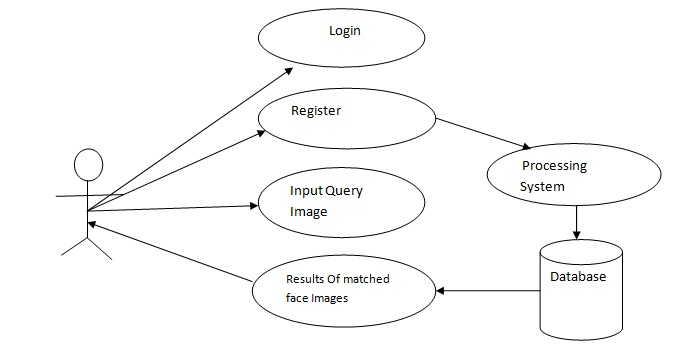
\includegraphics[height=250pt,width=435pt]{usecase.jpg}\\
\caption{UseCase Diagram}
\end{figure}

\newpage
\begin{itemize}
\item \textbf {Class Diagram}
\end{itemize}

\begin{figure}[ht!]
	\centering
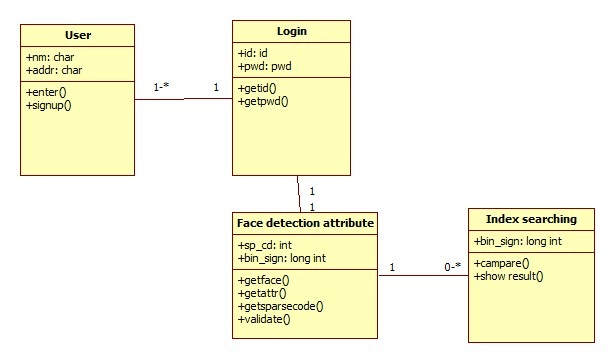
\includegraphics[height=250pt,width=435pt]{class1.jpg}\\
\caption{Class Diagram}
\end{figure}

\begin{itemize}
\item \textbf {Activity Diagram}
\end{itemize}

\begin{figure}[ht!]
	\centering
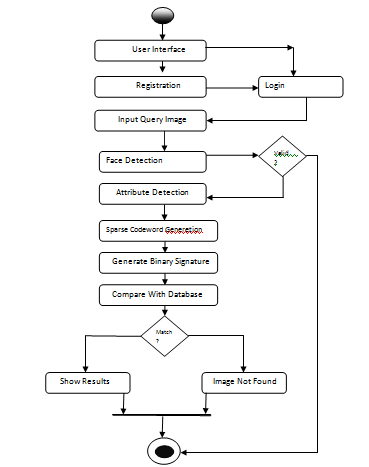
\includegraphics[height=300pt,width=435pt]{acti.png}\\
\caption{Activity Diagram}
\end{figure}
\newline\newline
\begin{itemize}
\item \textbf {Component Diagram}
\end{itemize}

\begin{figure}[ht!]
	\centering
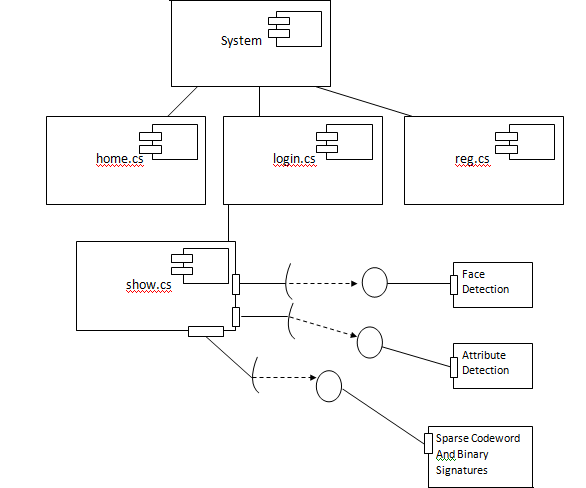
\includegraphics[height=350pt,width=435pt]{comp.png}\\
\caption{Component Diagram}
\end{figure}
\newpage

\begin{itemize}
\item \textbf {Sequence Diagram}
\end{itemize}

\begin{figure}[ht!]
	\centering
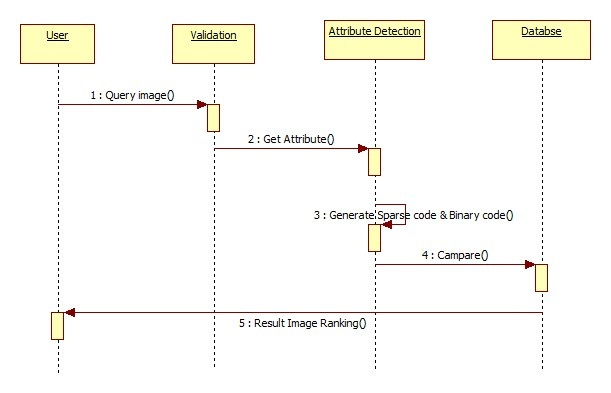
\includegraphics[height=300pt,width=300pt]{Seq.png}\\
\caption{Sequence Diagram}
\end{figure}



\begin{itemize}
\item \textbf {Deployment Diagram}
\end{itemize}

\begin{figure}[ht!]
	\centering
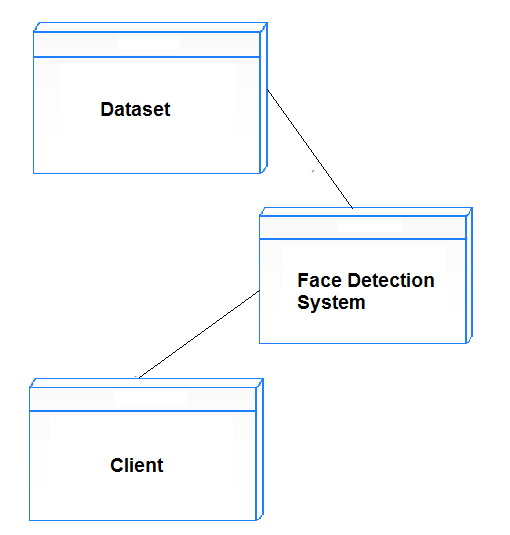
\includegraphics[height=250pt,width=300pt]{dep.png}\\
\caption{Deployment Diagram}
\end{figure}




\section{\normalsize{\textbf{Methods and Procedures}}}
\subsection{\normalsize{\textbf{Modules of the Project}}}
\begin{itemize}
\item \textbf{Face Detection and Attribute Detection:}\newline
This module detects Face from query image by applying Face detection algorithm. We apply another algorithm for attribute detection.
\end{itemize}
\begin{itemize}
\item \textbf{Attribute Enhanced sparse coding:}\newline
This module creates sparse codeword for every Database Image and query image and store for every image in database.
\end{itemize}
\begin{itemize}
\item \textbf{Face Image Retrieval Using Embedded Inverted Indexing:}\newline
This module is used for retrieving images form Database using binary Signature that are generated for every Image in database and Query image using sparse code words. So Indexing is used for Images in database which improves retrieval time and performance of software.
\end{itemize}
\subsection{\normalsize{\textbf{Detailed Flow of the Project}}}
\begin{figure}[ht!]
	\centering
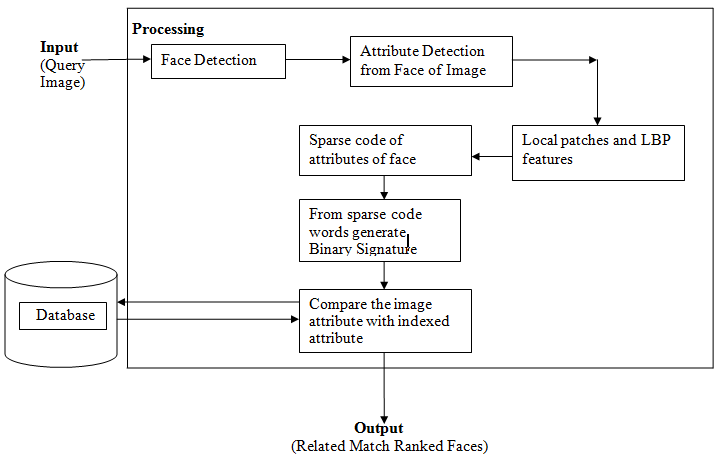
\includegraphics[height=250pt,width=300pt]{block1.png}\\
\caption{Block Diagram}
\end{figure}

\section{\normalsize{\textbf{Screen shots}}}
(decide in consultation with guide)
